\documentclass[a4paper,spanish,12pt]{article}
\usepackage[spanish]{babel}
\usepackage[utf8]{inputenc}
\usepackage[pdftex]{graphicx}
\usepackage{vmargin}
%\usepackage{algorithmic}
%\usepackage{float}
\usepackage{lastpage}
\usepackage{caratula}
\usepackage{algorithm}
\usepackage{algorithmic}
\usepackage{url}


%%%%%%%%%%%%%%%%%%%%%%%%%%%%%%%%%%%%%%%%%
% ECO Para jugar con el footer. 		%
\usepackage{fancyhdr}					%
%%%%%%%%%%%%%%%%%%%%%%%%%%%%%%%%%%%%%%%%%


%%\usepackage{hyphenat}
%%\exhyphenpenalty=10000
%%\hyphenpenalty=10000
\setmarginsrb{10mm}% left margin
{15mm}% top margin
{15mm}% right margin
{10mm}% bottom margin
{0mm}{20mm}{0mm}{30mm}% we needed -- related to headers and footers

%%%%%%%%%%
\pagestyle{fancy}
\fancyhf{}

\fancyhead[RO, CE]{Teor\'{i}a de las Comunicaciones}
%\fancyhead[LO, CE]{Grupo X}
\fancyfoot[C]{ Página \thepage\ de \pageref{LastPage} }

\renewcommand{\headrulewidth}{0.6pt}
\renewcommand{\footrulewidth}{0.6pt}

\newcommand{\ite}[3]{\textbf{if} #1 \textbf{then} \\ \hspace*{7mm}\vbox{#2} \\ \textbf{else} \\ \hspace*{7mm}\vbox{#3} \\ \textbf{fi} }
\newcommand{\itf}[3]{\textbf{if} #1 \textbf{then} \\ \hspace*{7mm}\vbox{#2} \\ \textbf{fi} \\ }
\newcommand{\whi}[2]{\textbf{while (} #1 \textbf{)} \\ \hspace*{7mm}\vbox{\noindent #2} }
\newcommand{\tades}[2]{\noindent\textbf{TAD} #1 \textbf{ES} #2 \\}
\newcommand{\punt}[1]{($\ast$#1)}
\newcommand{\fle}{$\rightarrow$}


%%%%%%%%%%

\begin{document}


%*************************************************************%
%                                                             %
% CARATULA                                                    %
%                                                             %
%*************************************************************%
    \materia{Teor\'{i}a de las Comunicaciones}

    \titulo{Trabajo Práctico 3}
  
    %\subtitulo{Tres problemas de programación}

    %\grupo{Grupo 255}

    \integrante{Alvarez Colombo, Santiago Javier}{719/10}{santialvarezcolombo@gmail.com}
    \integrante{Calderini, Nicol\'{a}s}{820/10}{calderini.nicolas@gmail.com}
    \integrante{Ferrari, Gast\'{o}n}{775/07}{gastonferrari5@hotmail.com}
    \maketitle
    
    \lhead{Trabajo Práctico 3}
    
%*************************************************************%
%                                                             %
% INFORME                                                     %
%                                                             %
%*************************************************************%

	\tableofcontents
	\newpage

\section{Abstract}
\indent En este trabajo práctico ejercitaremos las nociones del nivel de transporte estudiadas en la materia a través de la implementación y análisis de un protocolo sencillo llamado PTC. Para hacerlo, implementaremos un cliente para interactuar con el servidor provisto por la catedra.\\


\section{Palabras Clave}
PTC, transporte, protocolo.






\newpage

\newpage
\section{Introducción Teórica}
\subsection{PTC} 
\indent Extracto del enunciado del TP sobre que es el protocolo PTC.\\
\indent El protocolo que estudiaremos, PTC (Protocolo de Teoría de las
Comunicaciones), puede ubicarse dentro de la capa de transporte del modelo OSI
tradicional. Fue concebido como un protocolo de exclusivo uso didáctico que
permita lidiar en forma directa con algunas de las problemáticas usuales de la
capa de transporte: establecimiento y liberación de conexión, control de errores
y control de flujo.

\subsection{Capa de transporte}
\indent El nivel de transporte o capa de transporte es el cuarto nivel del
modelo OSI encargado de la transferencia libre de errores de los datos entre el
emisor y el receptor, aunque no estén directamente conectados, así como de
mantener el flujo de la red. Es la base de toda la jerarquía de protocolo. La
tarea de esta capa es proporcionar un transporte de datos confiable y económico
de la máquina de origen a la máquina destino, independientemente de la red de
redes física en uno. Sin la capa transporte, el concepto total de los protocolos
en capas tendría poco sentido.

\section{An\'alisis de entrop\'ia}


\indent Para este punto decidimos tomar como s\'imbolos de la fuente de informaci\'on a las direcciones IP de los nodos de una red de hogar.
Como modelo vamos a analizar los datos de diferentes maneras:

\subsubsection{Primera red (6 horas de capturas de paquetes):}

\begin{itemize}
 \item  IPs que realizaron consultas ARP:
\end{itemize}

\begin{tabular}{|l|l|l|l|l|}
  \hline
  S\'imbolo & Consultas & Probabilidad & Informaci\'on \\
  \hline
  192.168.0.105 & 99 & 0.0947368421053 & 3.39993060689 \\
  \hline
  192.168.0.104 & 28 & 0.0267942583732 & 5.22193230491 \\
  \hline
  192.168.0.1 & 415 & 0.397129186603  & 1.33231970073 \\
  \hline
  192.168.0.101 & 448 & 0.428708133971 & 1.22193230491 \\
  \hline
  192.168.0.100 & 1 & 0.000956937799043 & 10.029287227 \\
  \hline
  192.168.0.103 & 11.0 & 0.0105263157895 & 6.56985560833 \\
  \hline
  192.168.0.102 & 26.0 & 0.0248803827751 & 5.32884750883 \\
  \hline
  0.0.0.0 & 17.0 & 0.0162679425837 & 5.94182438572 \\
  \hline
\end{tabular}

\\ \ \\ \ \\ 
Entrop\'ia de la fuente:\\
$H(S) = -\sum_{s \in S} P(s) I(s)$\\
$H(S) = 1.82297065237$\\

En este caso la IP que realiz\'o m\'as consultas ARP fue 192.168.0.101. 
La segunda fue 192.168.0.1 (router), \'esto es l\'ogico considerando que el router es el encargado de distribuir todo el tr\'afico de la red a los nodos correspondientes por lo que su tabla
de direcciones macs tiene que estar correctamente actualizada el mayor tiempo posible.

\newpage

\begin{tabular}{|l|l|l|l|l|}
  \hline
  S\'imbolo & Respuestas & Probabilidad & Informaci\'on \\
  \hline
  192.168.0.105 & 506 & 0.85472972973 & 0.226459790935 \\
  \hline
  192.168.0.101 & 24 & 0.0405405405405 & 4.62449086491 \\
  \hline
  192.168.0.1 & 62 & 0.10472972973 & 3.25525705524\\
  \hline
\end{tabular}\\

\\ \ \\ \ \\ 
Entrop\'ia de la fuente\\
$H(S) = -\sum_{s \in S} P(s) I(s)$\\
$H(S) = 0.721963466885$\\

En este caso la IP 192.168.0.105 fue la que m\'as veces contest\'o los pedidos sobre su MAC, aumentando su probabilidad. Como se puede observar, la informaci\'on
aportada por esta IP es considerablemente m\'as baja que la aportada por las dem\'as que poseen menor probabilidad e incluso m\'as baja que la entrop\'ia de la red.\\\\

\newpage
\begin{itemize}
 \item IPs por las que se realizaron consultas ARP:\\
\end{itemize}

\begin{tabular}{|l|l|l|l|l|}
  \hline
  S\'imbolo & Consultas & Probabilidad & Informaci\'on \\
  \hline
  169.254.37.204 & 3.0 & 0.00287081339713 & 8.44432472625\\
  \hline
  192.168.0.105 & 506.0 & 0.484210526316 & 1.04629365227\\
  \hline
  192.168.0.104 & 52.0 & 0.0497607655502 & 4.32884750883\\
  \hline
  169.254.255.255 & 10.0 & 0.00956937799043 & 6.70735913208\\
  \hline
  192.168.0.1 & 88.0 & 0.0842105263158 & 3.56985560833\\
  \hline
  192.168.0.101 & 30.0 & 0.0287081339713 & 5.12239663136\\
  \hline
  192.168.0.100 & 316.0 & 0.302392344498 & 1.72550647879\\
  \hline
  192.168.0.103 & 18.0 & 0.0172248803828 & 5.85936222553\\
  \hline
  192.168.0.102 & 22.0 & 0.0210526315789 & 5.56985560833\\
  \hline
\end{tabular}\\
\\ \ \\ \ \\ 
Entrop\'ia de la fuente\\
$H(S) = -\sum_{s \in S} P(s) I(s)$\\
$H(S) = 1.99810125093$\\

En este caso la IP m\'as consultada en la red fue la 192.168.0.105. Al igual que en el punto anterior por consecuencia de su alta probabilidad de aparecer en la fuente, su informaci\'on no supera a la entrop\'ia que ofrece la red.



\newpage
\section{Resultados}
\indent Para probar el protocolo, armamos archivos de 1kb, 5kb, 10kb, 50kb, 100kb, 200kb y
500kb. El servidor y el cliente se encuentran en distintos host en la misma LAN sobre Wi-Fi la cual presenta un RTT de aproximadamente 2ms entre ambos hosts. Para
tomar los tiempos y comprobar el correcto funcionamiento del protocolo, usamos
el wireshark.\\
\indent Para tener mediciones mas aproximadas a la realidad, tomamos el promedio de 10 mediciones.\\

\subsection{Tiempo de transmisión}
\indent En este primer gráfico presentamos el tiempo de transmisión de los archivos, usando SEND\_WINDOWs de 1, 10, 15 y 20.

\begin{figure}[h]
  \centering                                                       
          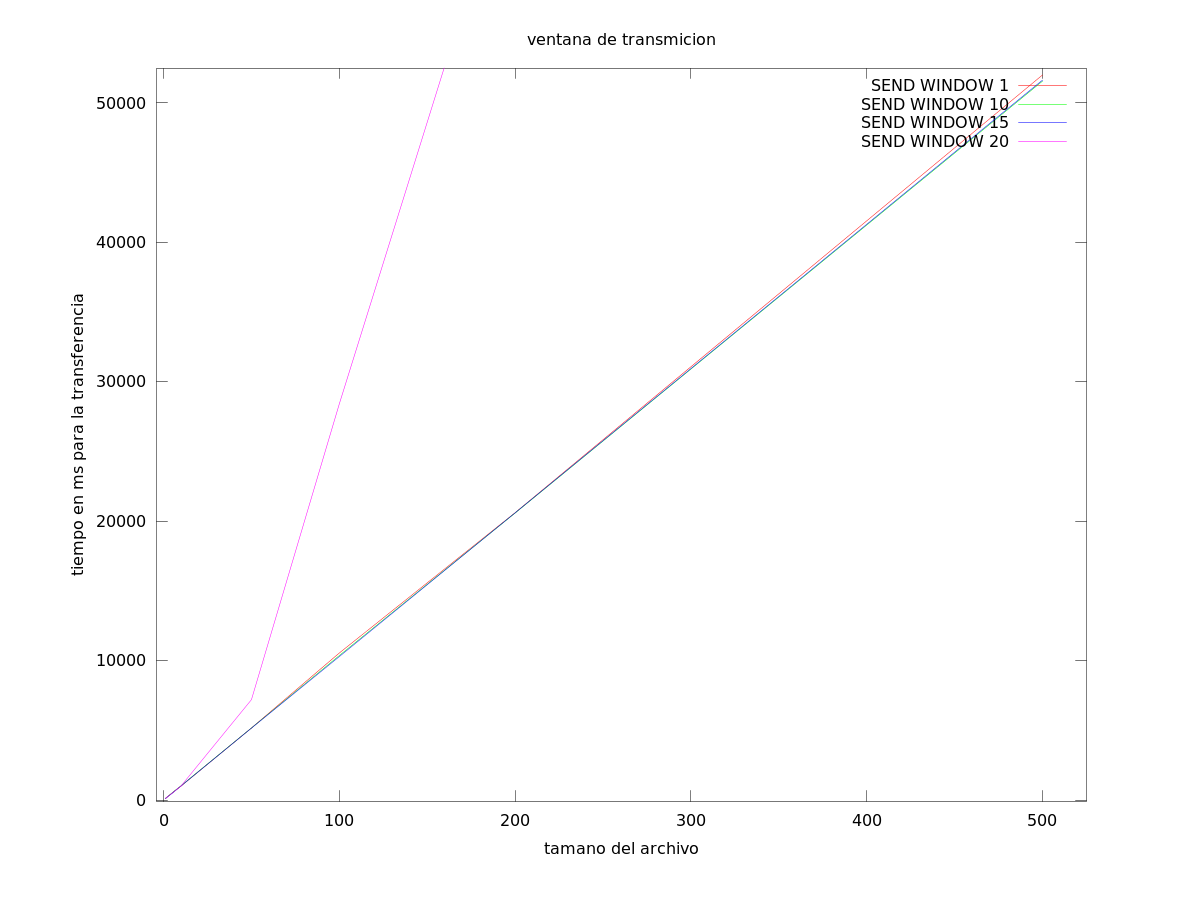
\includegraphics[width=500pt]{./datos/graf.png}
          \caption{Tiempo de transmisión}
          \label{fig:tt}
\end{figure}

\clearpage
\indent En el gráfico podemos observar como el tiempo de transmisión usando
ventanas de 1, 10 y 15, es muy similar. En cambio, cuando usamos una ventana de
20, es notable la diferencia en el tiempo que tarda en enviarse el
archivo. Esto se debe a la cantidad de timeouts que ocurren al utilizar este tamaño de ventana.\\

\subsection{Velocidad de Transferencia}
\indent En este segundo gráfico presentamos la velocidad de transmisión (en kb\/s) de la transmisión de los archivos, usando SEND\_WINDOWs de 1, 10, 15 y 20.

\begin{figure}[h]
  \centering                                                       
          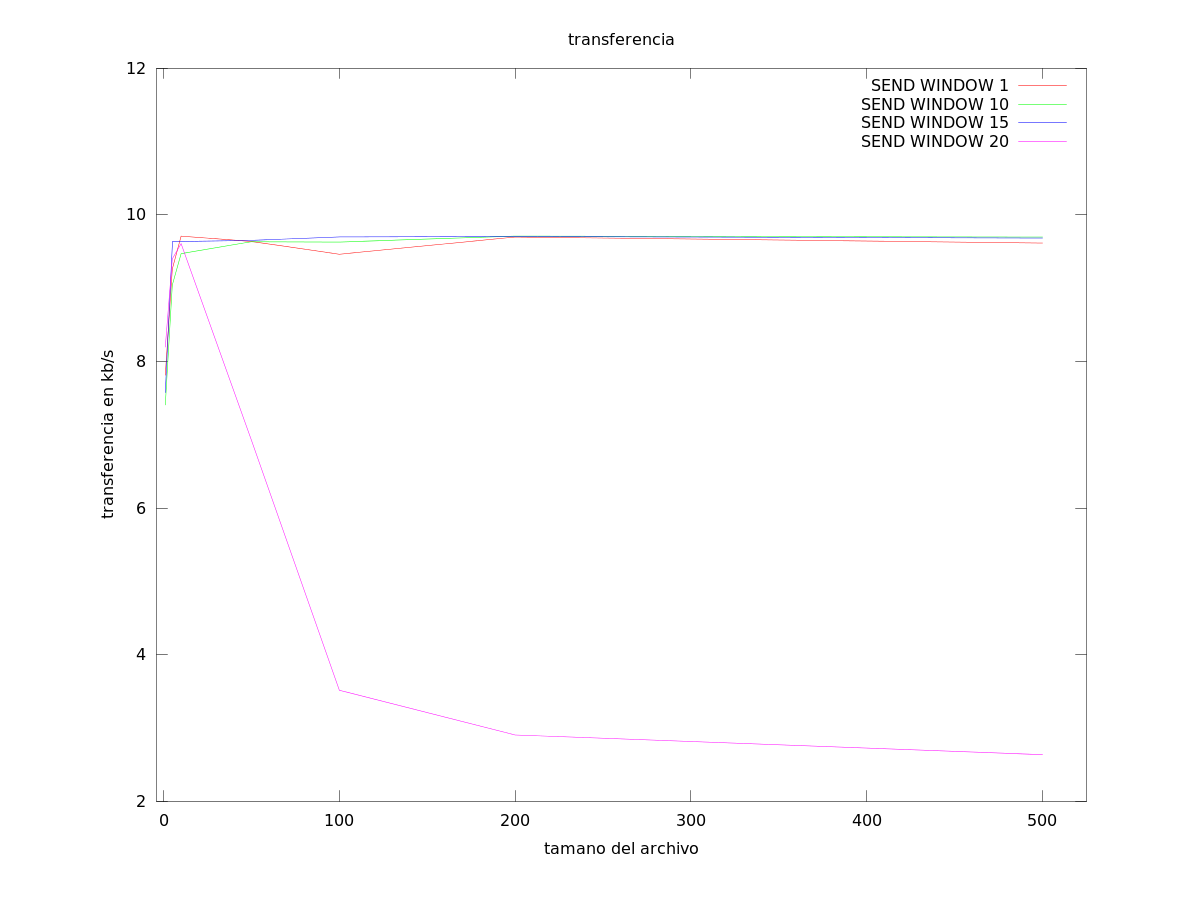
\includegraphics[width=550pt]{./datos/transferencia.png}
          \caption{Tiempo de transmisión}
          \label{fig:vt}
\end{figure}

\clearpage
\indent Al igual que en el gráfico anterior, podemos observar la gran diferencia
que existe en la velocidad de transmisión cuando la ventana de emisión crece.\\
\indent La velocidad se mantiene estable con ventanas de 1,
10 y 15, pero cuando usamos una ventana de 20, la velocidad
tiende a caer mucho a medida de que aumenta el tamaño del archivo.\\
\indent Si comparamos este gráfico con el anterior, se ve claramente como al
ser menor el throughput, el tiempo de transmisión es mucho mayor.\\

\subsection{Cantidad de Timeouts}
\indent En esta sección presentamos la cantidad de timeouts que tuvieron en promedio el envío de los archivos.\\
\begin{center}
   \begin{tabular}{| c | c | c | c | c |}
    \hline
    Tamaño del archivo/SEND\_WINDOW & 1 & 10 & 15 & 20\\
    \hline
    1kb & 0 & 0 & 0 & 0 \\
    \hline
    5kb & 0 & 0 & 0 & 0 \\
    \hline
    10kb & 0 & 0 & 0 & 0\\
    \hline
    50kb & 0 & 0 & 0 & 5\\
    \hline
    100kb & 0 & 0 & 0 & 14\\
    \hline
    200kb & 0 & 0 & 0 & 34\\
    \hline
    500kb & 0 & 0 & 0 & 94\\
    \hline
  \end{tabular}
\end{center}

\indent De igual manera que en las 2 secciones anteriores, podemos observar la gran
diferencia que hay entre las ventanas, en este caso, con respecto a los
timeout.\\
\indent Vemos que con ventanas de 1, 10 y 15, no tuvimos timeout en ninguno de
los archivos que mandamos. En cambio, vemos que con la ventana en 20, los
archivos mas chicos tampoco tuvieron timeout, cuando los archivos mas grandes
empiezan a presentar cada vez mas timeouts. Los timeouts se dan ya que los paquetes encolados en la cola de retransmisión del emisor se les acaba el $RETRANSMISSION\_TIMEOUT$ dado que los acks que se reciben del receptor no llegan lo suficientemente rápido para evitar que se acabe dicho tiempo para el paquete. Si seguimos aumentando el send window a tamaños mayores a 20 solo empeoraríamos la perfomance ya que al producirse un timeout se aplica una política de retransmisión de GoBackN lo que implica que una mayor cantidad de paquetes se deben retransmitir.\\

%\subsection{Tiempo de transmisión}
%\indent En el gráfico podemos observar como el tiempo de transmisión usando
%ventanas de 1, 10 y 15, es muy similar. En cambio, cuando usamos una ventana de
%20, es notable la diferencia en el tiempo que tarda en enviarse el
%archivo. Esto se debe a la cantidad de timeouts que ocurren al utilizar este tamaño de ventana.\\
%
%\subsection{Velocidad de Transferencia}
%\indent Al igual que en el gráfico anterior, podemos observar la gran diferencia
%que existe en la velocidad de transmisión cuando la ventana de emisión crece.\\
%\indent La velocidad se mantiene estable con ventanas de 1,
%10 y 15, pero cuando usamos una ventana de 20, la velocidad
%tiende a caer mucho a medida de que aumenta el tamaño del archivo.\\
%\indent Si comparamos este gráfico con el anterior, se ve claramente como al
%ser menor el throughput, el tiempo de transmisión es mucho mayor.\\
%
%\subsection{Cantidad de TimeOut}
%\indent Al igual que en las 2 secciones anteriores, podemos observar la gran
%diferencia que hay entre las ventanas, en este caso, con respecto a los
%timeout.\\
%\indent Vemos que con ventanas de 1, 10 y 15, no tuvimos timeout en ninguno de
%los archivos que mandamos. En cambio, vemos que con la ventana en 20, los
%archivos mas chicos tampoco tuvieron timeout, cuando los archivos mas grandes
%empiezan a presentar cada vez mas timeouts. Los timeouts se dan ya que los paquetes encolados en el buffer del emisor se les acaba el ttl dado que los acks que se reciben del receptor no llegan lo suficientemente rápido para evitar que se acabe dicho tiempo para el paquete. Si seguimos aumentando el send window a tamaños mayores a 20 solo empeoraríamos la perfomance ya que al producirse un timeout se aplica una política de retransmisión de GoBackN lo que implica que una mayor cantidad de paquetes se deben retransmitir.


\newpage
\section{Discusión}
\subsection{Análisis del tiempo de transmisión}
\indent En el gráfico podemos observar como el tiempo de transmisión usando
ventanas de 1, 10 y 15, es muy similar. En cambio, cuando usamos una ventana de
20, se nota la abismal diferencia en el tiempo que tarda en enviarse el
archivo. Esto se debe claramente a la cantidad de timeouts que produce utilizar este tamaño de ventana.\\
\indent Para poder mostrar con mas énfasis esta gran diferencia que existe en el
tiempo de transmisión cuando crece la ventana, tratamos de probar con tamaños de
ventana mas grandes, pero no obtuvimos resultados, dado que el protocolo no
soportaba esa cantidad de datos en vuelo y nunca llegaba a destino el archivo.\\

\subsection{Velocidad de Transferencia}
\indent Al igual que en el gráfico anterior, podemos observar la gran diferencia
que existe en la velocidad de transmisión cuando la ventana de emisión crece.\\
\indent La velocidad se mantiene estable con ventanas de 1,
10 y 15, pero cuando usamos una ventana de 20, la velocidad
tiende a caer mucho a medida de que aumenta el tamaño del archivo.\\
\indent Si comparamos este gráfico con el anterior, se ve claramente como al
ser menor el throughput, el tiempo de transmisión es mucho mayor.\\

\subsection{Cantidad de TimeOut}
\indent Al igual que en las 2 secciones anteriores, podemos observar la gran
diferencia que hay entre las ventanas, en este caso, con respecto a los
timeout.\\
\indent Vemos que con ventanas de 1, 10 y 15, no tuvimos timeout en ninguno de
los archivos que mandamos. En cambio, vemos que con la ventana en 20, los
archivos mas chicos tampoco tuvieron timeout, cuando los archivos mas grandes
empiezan a presentar cada vez mas timeouts. Los timeouts se dan ya que los paquetes encolados en el buffer del emisor se les acaba el ttl dado que los acks que se reciben del receptor no llegan lo suficientemente rápido para evitar que se acabe dicho tiempo para el paquete. Si seguimos aumentando el send window a tamaños mayores a 20 solo empeoraríamos la perfomance ya que al producirse un timeout se aplica una política de retransmisión de GoBackN lo que implica que una mayor cantidad de paquetes se deban retransmitir.

\newpage
\section{Conclusiones}
\indent Como conclusión del TP, nos gustaría resaltar las particularidades que
encontramos en el protocolo.\\
\indent Creemos que al tener una ventana de recepción de 1, el emisor esta muy
restringido en cuanto al valor de su ventana de emisión. Esto genera que para
valores de la ventana de emisión que superan 20, se genere tal cuello de botella
en el receptor, que el protocolo deja de funcionar de manera eficiente y aceptable. También provoca que los tamaños de ventana de emisión con valores menores a 20 se comporten y presenten una performance casi idéntica ya que la ventana de recepción de tamaño 1 no permite aprovechar este aumento.\\
\indent 

\newpage
\section{Bibliografia}
\begin{itemize}
 \item \url{http://es.wikipedia.org/wiki/Capa_de_transporte}
 \item Tanenbaum, A. Computer Networks, 3ra Ed. Capítulo 3: páginas 207-213.
\end{itemize}




 
\end{document}